\part{Introduction}%
This part of the of the document describes the content of the document and how it should be used, and the changes from version 1.0 of the thesis template.
\chapter{About the template}
\section{What's in this package?}

\begin{definitionlist}
    \item{Example.tex} An example of new and redefined commands.
    \item{Instruction.tex} This file.
    \item{ProblemsAndSolutions.tex} Possible problems and solutions.
    \item{References.bib} An example of a reference file. 
    \item{Thesis.pdf, Thesis.ps \& Thesis.dvi} The result of compiling Thesis.tex.
    \item{Thesis.tex} A document template for using the UUThesisTemplate class.
    \item{UU\_ logo\_ pc\_ 42.eps} Title page logo in EPS format.
    \item{UU\_ logo\_ pc\_ 42.pdf} Title page logo in PDF format.
    \item{UUThesisTemplate.cls} A document class, based on the standard class \code{book}, that redefines commands and presets in order to produce a document following the guidelines for theses.   
\end{definitionlist}

\section{Instructions}
The document template consists of one main file, \emph{Thesis.tex}, which implements the UUThesisTemplate document class and includes a few packages, to make sure the fonts are set up correctly. The thesis may be split into one or several chapter files to be included in the main matter of the Thesis.tex file. All the normal commands and environments defined in the standard class book can be used, although some of them have been redefined for typographical reasons. 

\subsection{New environments}
A number of list environments have been added to the template. These are:
\begin{tabbing}
\hspace{4cm}\=\kill
numberedlist \> Enumeration adjusted to numbers 1--9.\\
numberedlist-indent \> Same as \code{numberedlist} but indented.\\
bulletlist \> Bullet list based on itemize.\\
bulletlist-indent \> Same as \code{bulletlist} but indented.\\
romanlist \> Enumeration with roman numerals.\\
romanlist-indent \> Same as \code{romanlist} but indented.\\
simplelist \> A simple list.\\
simplelist-indent \> Same as \code{simplelist} but indented.
\end{tabbing}

\section{Changes from earlier versions of this template}
\begin{bulletlist} 
\item Complete rewrite to ease usage and maintainance.
\item Now applied as a document class instead of a package.
\item New environments, e.g. \code{listofpapers} and \code{abstract}, added.
\item New commands, e.g. \code{\textbackslash makehalftitle} and \code{\textbackslash titlepagelogo}, added.
\item Compability issues with XeLaTeX have been resolved.
\end{bulletlist} 

\section{Important note}
This template may used with a PDFLaTeX or XeLaTeX driver to produce the output as a PDF file, which also allow you to include figures in formats such as JPEG, PNG or PDF. EPS files and other unsupported formats have to be converted before inclusion\footnote{Command-line tools like \emph{ps2pdf} or \emph{convert} can do this as well as the application \emph{Preview} for Mac OS X.}. Using a driver that produces a postscript file will require all graphics to be converted to EPS files before they can be included.   

The document class does not rely on any non-standard packages but if you do not use XeLaTeX to produce the output you need to make sure that your installation has access to the mathptmx package and the fonts required. Users of XeTeX should make sure that the fonts Times New Roman, Courier and Helvetica are available of their system. 

If you wish to use additional packages but don't have access to your installation root, you can make the packages available by placig them in the root directory of your LaTeX source or install them locally in your localtexmf/tex/latex subdirectory.
 
\subsection{Fonts}
PDF files created from LaTeX usually don't include embedded fonts. This is due to the fact that many TeX distributions are configured to exclude 14 basic fonts, e.g. Times and Helvetica. Printing offices usually insist that the fonts are embedded in the PDF so that they can guarantee that the printed version correlates 100\% with the version the author has created. Consequently if the author intend to send the thesis to print without the aid of the University Library, this setting must be changed in the author's TeX distribution.



\subsubsection{How do I know that my fonts are embedded?}
In Acrobat Reader, select File\(\rightarrow\)Document properties\(\rightarrow\)Fonts. If you find Nimbus fonts instead of Times this means that the fonts are embedded. If you use another font i.e. Fourier or Utopia, make sure that there is a \emph{yes} in the embedded column of this dialog.

    \begin{figure}[!ht]
    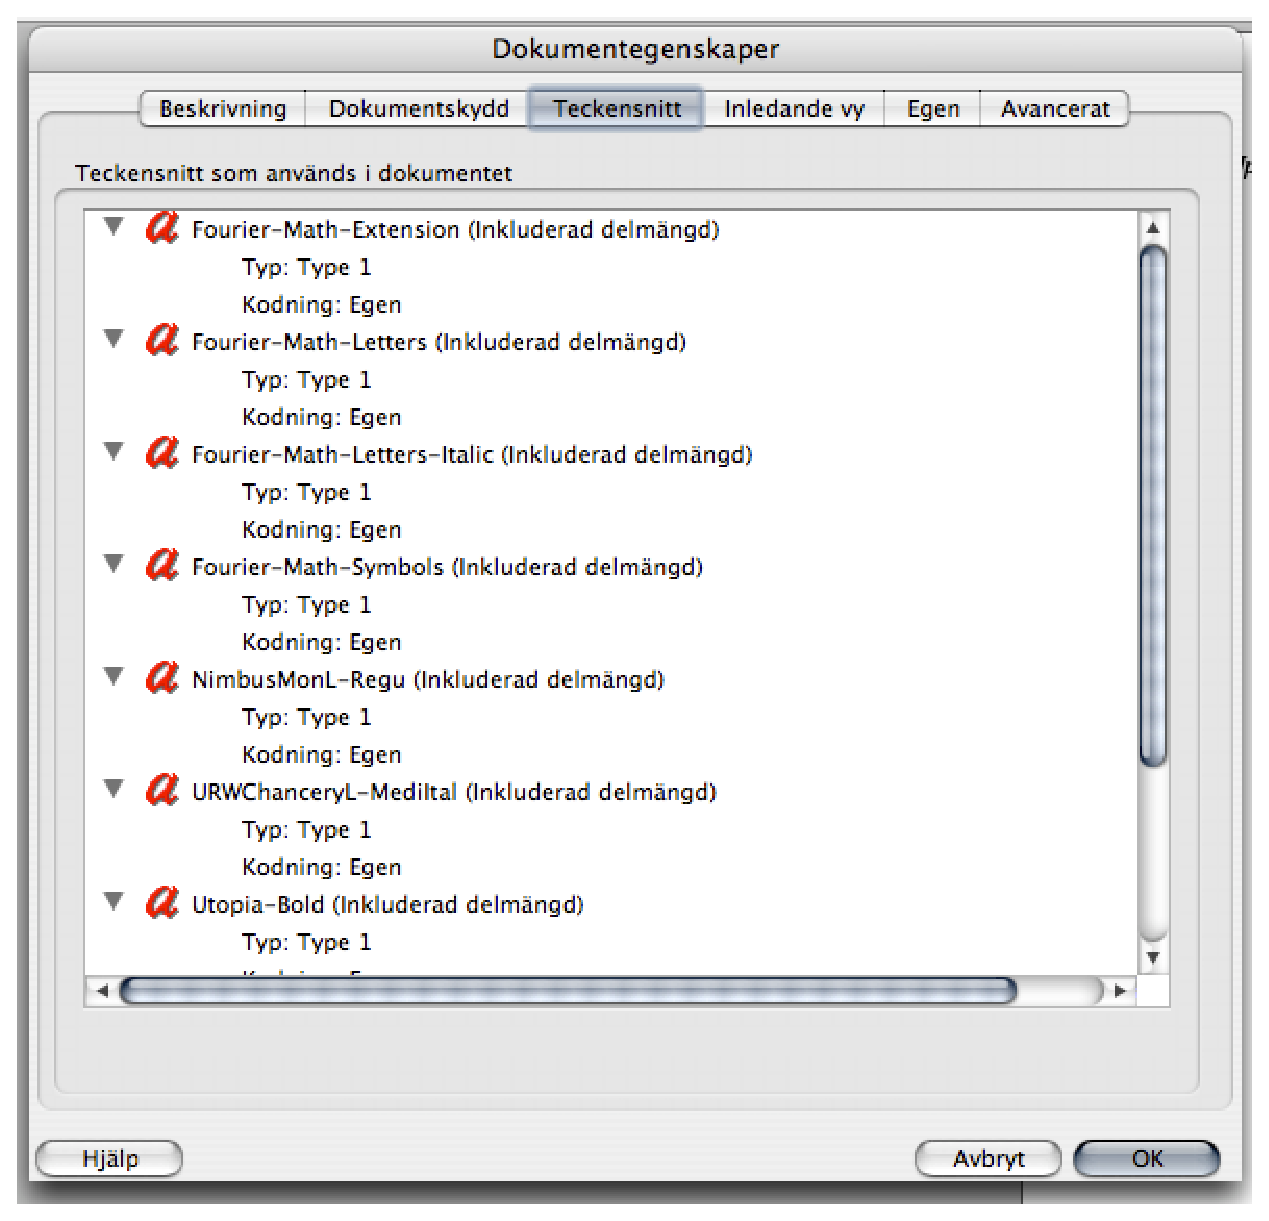
\includegraphics[width=12cm]{Example/Fonts}
	\caption{Acrobat document properties and fonts display} 
    \end{figure} 

\vspace{\baselineskip}
\noindent Please send any questions, comments or macro contributions to\\espik@ub.uu.se.

\chapter[About authoring a dissertation at Uppsala University]{About authoring a dissertation \linebreak[3]at Uppsala University}
In order to ensure a uniform layout for, and simplify the making of the dissertations published in the Acta series of Uppsala
University, Publishing and Graphic Services has created a document template for \LaTeXe{}. This template also ensures that it will be possible to save a digital version of the dissertation for long-time storage and enable a full-text search in the dissertation
database. You find the template "Avhandlingsmall" at http://www.ub.uu.se/pgsen.
\section{Typography}
The template is based on the typography that the Editorial Office at Uppsala University applies to Acta
monographs. The page format is S5 (165 x 242 mm), and the font used throughout is Times with a body text type size of 11 points. The left and right margins are 22,5 mm, and the top and bottom margins are 20 mm.
\section{Outline}
A comprehensive summary should include the following parts in the following order:
\begin{bulletlist}
    \item Title Page (produced by Publishing and Graphic Services).
    \item Abstract/Imprint page (produced by Publishing and Graphic Services all\-though a demo comes with the tempalate).
    \item Dedication page. Optional.
    \item List of Papers.
    \item Table of Contents.
    \item Introduction/Background (the first chapter; the first page to be paginated using Arabic numerals).
    \item Chapter 1 \ldots n.
    \item Summary in Swedish (Mandatory for all Tek-Nat students).
    \item Acknowledgments.
    \item References/Bibliography.
    \item Acta Back Cover (produced by Publishing and Graphic Services).
\end{bulletlist}
\vspace{1\baselineskip}
A monograph should include the following parts in the following order:

\begin{bulletlist}
    \item Half-title page.
    \item Title Page.
    \item Abstract/Imprint page (produced by Publishing and Graphic Services all\-though a demo comes with the template).
    \item Dedication page. Optional.
    \item Table of Contents.
    \item Introduction/Background (the first chapter; the first page to be paginated using Arabic numerals).
    \item Chapter 1 \ldots n.
    \item Summary in Swedish (Mandatory for all Tek-Nat students).
    \item Acknowledgments.
    \item References/Bibliography.
\end{bulletlist}
\vspace{1\baselineskip}
\noindent The front matter (the sequence of pages from the half-title page or the title page up to the table of contents) is never paginated. The sequence from Chapter 1 up to References/Bibliography is paginated using Arabic numerals. 
